\documentclass[tikz,border=10pt]{standalone}

\usepackage{xcolor}
\usetikzlibrary{
    arrows.meta,
    positioning,
    fit,
    backgrounds,
    shapes.geometric
}

\begin{document}

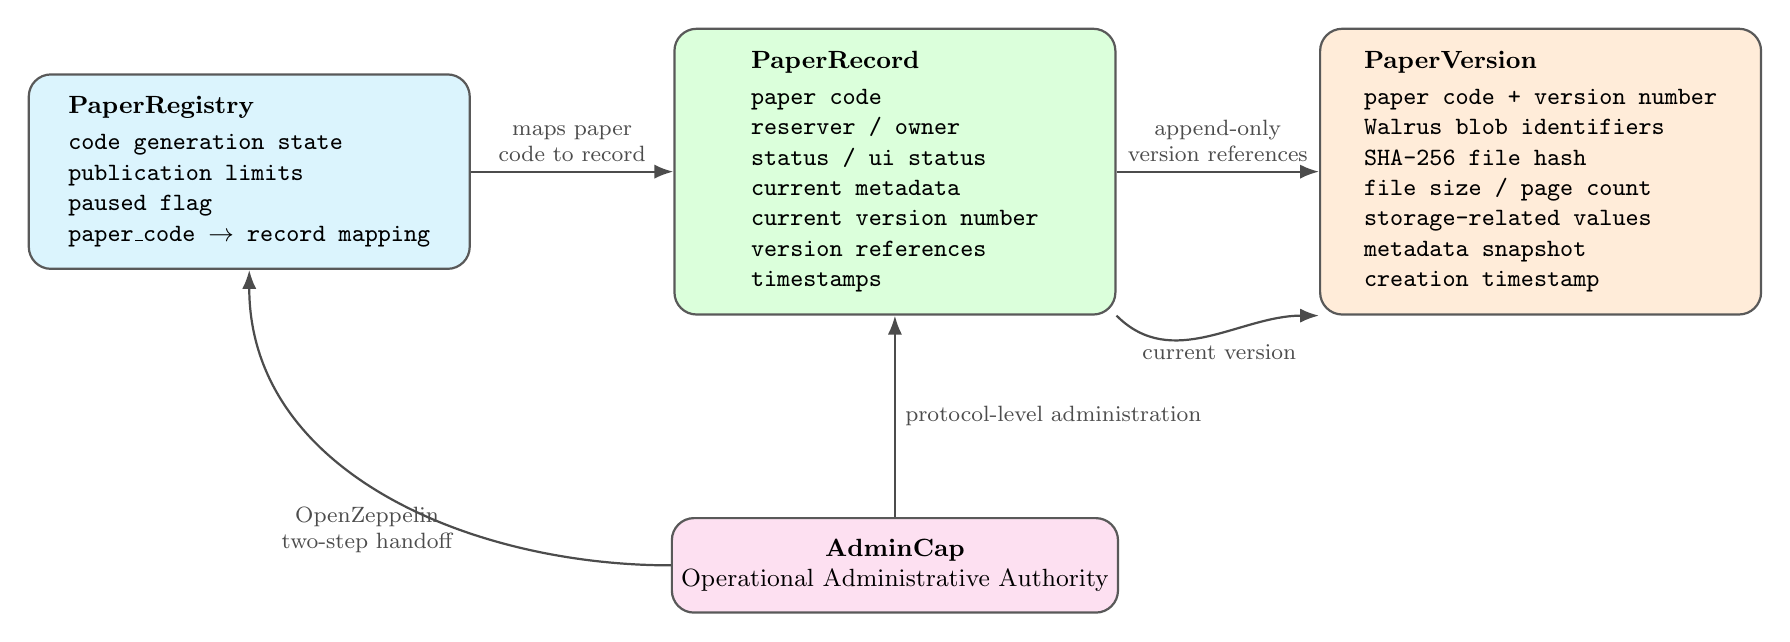
\begin{tikzpicture}[
    font=\small,
    entity/.style={
        rectangle,
        rounded corners=8pt,
        draw=black!65,
        thick,
        align=left,
        minimum width=5.6cm,
        minimum height=2.2cm,
        fill=white,
        inner sep=8pt
    },
    capbox/.style={
        rectangle,
        rounded corners=8pt,
        draw=black!65,
        thick,
        align=center,
        minimum width=3.6cm,
        minimum height=1.2cm,
        fill=white
    },
    arrow/.style={
        -{Latex[length=2.4mm,width=1.8mm]},
        thick,
        draw=black!70
    },
    note/.style={
        font=\footnotesize,
        align=center,
        text=black!70
    }
]

% =========================================================
% Main objects
% =========================================================
\node[entity, fill=cyan!14] (registry) at (0,0) {
\textbf{PaperRegistry}\\[2pt]
\texttt{code generation state}\\
\texttt{publication limits}\\
\texttt{paused flag}\\
\texttt{paper\_code $\rightarrow$ record mapping}
};

\node[entity, fill=green!14] (record) at (8.2,0) {
\textbf{PaperRecord}\\[2pt]
\texttt{paper code}\\
\texttt{reserver / owner}\\
\texttt{status / ui status}\\
\texttt{current metadata}\\
\texttt{current version number}\\
\texttt{version references}\\
\texttt{timestamps}
};

\node[entity, fill=orange!15] (version) at (16.4,0) {
\textbf{PaperVersion}\\[2pt]
\texttt{paper code + version number}\\
\texttt{Walrus blob identifiers}\\
\texttt{SHA-256 file hash}\\
\texttt{file size / page count}\\
\texttt{storage-related values}\\
\texttt{metadata snapshot}\\
\texttt{creation timestamp}
};

\node[capbox, fill=magenta!12] (admincap) at (8.2,-5.0) {
\textbf{AdminCap}\\
Operational Administrative Authority
};

% =========================================================
% Main relations
% =========================================================
\draw[arrow] (registry) -- node[above, note] {maps paper\\code to record} (record);
\draw[arrow] (record) -- node[above, note] {append-only\\version references} (version);
\draw[arrow] (admincap) -- node[right, note] {protocol-level administration} (record);

% =========================================================
% Version semantics




% 

% =========================================================
% Ownership / lifecycle labels
% =========================================================
\draw[arrow] (record.south east) to[out=-45,in=180] node[pos=0.55, below, note] {current version} (version.south west);

\draw[arrow] (admincap) to[out=180,in=-90] node[pos=0.35, left, note] {OpenZeppelin\\two-step handoff} (registry.south);

% =========================================================


\end{tikzpicture}

\end{document}
